%%%Preamble
% packages and document class
\documentclass[a4paper, 12pt]{article}
\usepackage[utf8]{inputenc}
\usepackage{biblatex}
\usepackage{geometry}
\usepackage{authblk}
\usepackage{lineno}
\usepackage{graphicx}

% page format
\geometry{left = 3cm, top = 3cm, bottom = 2cm, right = 2cm}
\linespread{2.0}

% article basic infos
\title{\vspace{-1.0cm} \line(1,0){450} \\From mutualism to antagonism: the coevolutionary influence of  context-dependent interactions in mutualistic networks\\\line(1,0){450}}

\author[1]{Lucas A. Camacho}
\author[2]{Paulo Roberto Guimarães Junior}
\date{}
\affil[1,2]{Departamento de Ecologia, Universidade de São Paulo, Rua do Matão, travessa 14, nº 321, Cidade Universitária, São Paulo - SP, CEP: 05508-090, Brasil.}


%%%Document begins
\begin{document}

\begingroup
\linespread{1.0}
\maketitle
\endgroup

\section{Introduction}
\linenumbers
Coevolution, the reciprocal evolutionary change between interacting species, is a main force influencing the diversity of species and the organization of ecological interactions in the community. The interactions structure (who interacts with whom) dictates which species are coevolving in the community. Thus, coevolution is a process that molds and is molded by ecological interactions. The most conspicuous known patterns of coevolution are on species traits related to ecological interactions like plants and herbivores, pollination or seed dispersal.

Historically, the empirical evidences of coevolution thrilled several worldwide known naturalists to describe the genetic and ecological mechanisms that drive coevolution and, consequently, influences the ecological interactions between species in communities. Daniel Janzen described a high specialized mutualistic interaction formed by coevolution between the acacia ant (\textit{Pseudomyrmex ferruginea}) and the bullhorn acacia (\textit{Acacia cornigera}). In this system, the ant lives exclusively in structures produced by the plant called domatia and repeal possible herbivores that may attack the plants. In this way, the ant has his colony guaranteed and the plant repeal unwanted visitors. Also, Fritz Müller studied the coloration patterns of neotropical butterflies wings and propose the first mathematical model to show how these patterns emerge by coevolution.

Systems of coevolution between two species  grounded the studies of how several species can coevolve in nature. Several species implies in several reciprocal evolutionary changes happening at the same time. Thus, coevolution process depends on how the ecological interactions are distributed in the community. A problem that emerge is how to account this several reciprocal evolutionary changes at once. An possible approach to solve this issue is use network theory. Networks are representations of species and the interactions between these species in the community. The use of networks of interactions enable the investigation of how different evolutive process form phenotipic pattern of species. Using the networks approach, we now know that coevolution in mutualistic networks of interactions lead to trait complementarity of species that interact. In antagonisms otherwise, the selection intensity acting on a prey and the predator can create coevolutionary arm's race. This different coevolutionary dynamics can reorganize the interactions structure in time, generating for example, temporal variation in species traits between interacting species.

The species traits that will be favoured by natural selection, the interaction network structure and the path of the coevolution process rely on the costs and benefits associated with different interaction outcomes. For example, mutualisms shows a higher benefit compared to the cost for both interacting species. If so, the efficiency of interaction will be higher in species with similar traits, where the species that has the higher proportion of interactions will order the trait complementarity of other species generating a particular coevolution process. Else, antagonism interactions shows a higher benefit than the cost for a predator or parasite and a low benefit than the cost for the prey or host. Considering now an antagonism network of interactions, explorer species that has explored species similar traits will be favoured. Otherwise, the higher explored trait difference than the explorer, better for the explored species, generating an arm's race coevolution dynamics. Despite the actual knowing of how these interaction outcomes will influence coevolution, there is a lack of knowledge on how these two outcomes in the same network can influence the coevolution process and the structure of interaction in the community.

Despite the utility of classifying the interactions by their costs and benefits, these costs and benefits are not fixed. In fact, there is growing evidence quantifying the outcomes variation of interactions in space and time. In the ant-plant system exemplified, a low abundance of acacia ants caused by external factors of the plant (\textit{i.e.} temperature, rainfall) can cause a low herbivore repealing efficiency. In this scenario, is possible that the production cost of domatia for the plant could be higher than the benefits from the ants. In this way, this interaction between the plant and the ant can pass from a mutualism to an antagonism, which the ant is benefited and the plant has higher cost than benefit. Considering that different communities can have different frequencies of mutualism/atagonism, interaction outcomes changing in time and space contributes to the mosaic of coevolution, generating distinct trait patterns of species and heterogeneous interaction networks and ecological communities. The interactions outcomes which vary in space or time because of biotic and abiotic factors are called context-dependent interactions.

The shift in interaction outcomes between mutualism and antagonism caused by the context-dependency creates networks that has both antagonism and mutualism outcomes together. Considering that the trait changing path of these two dynamics are pretty different, the coevolutionary dynamics will be favoured by these two types of interactions. More than that, the interactions outcomes varying in time in the same community can influence species more in a mutualism or antagonism-like dynamic, depending on the network structure of interactions and how these outcomes shifts happen in time. In other words, the context dependency of interactions changing the interactions outcomes generates changes in the coevolutionary dynamics of species, changing the trait diversity of species and the interaction structure of the community in unknown ways. IMPORTANCIA DE CONTEXT DEPENDENT This should not be ignored if we want a higher understanding of the ecosystems function and diversity. 

Here, we use a single trait mathematical model, theoretical and empirical networks of species interactions and computer simulations to fill the gap of merge two different interaction outcomes in one network of interactions and consider the context-dependency of these interactions outcomes. Specifically, we are trying to answer two main questions: \textit{i)} how mutualism and antagonism outcomes in the same network changes the coevolutionary process? \textit{ii)} how context-dependent interactions influences the coevolutionary process?

% add figure 1
\begin{figure}
\linespread{1.0}

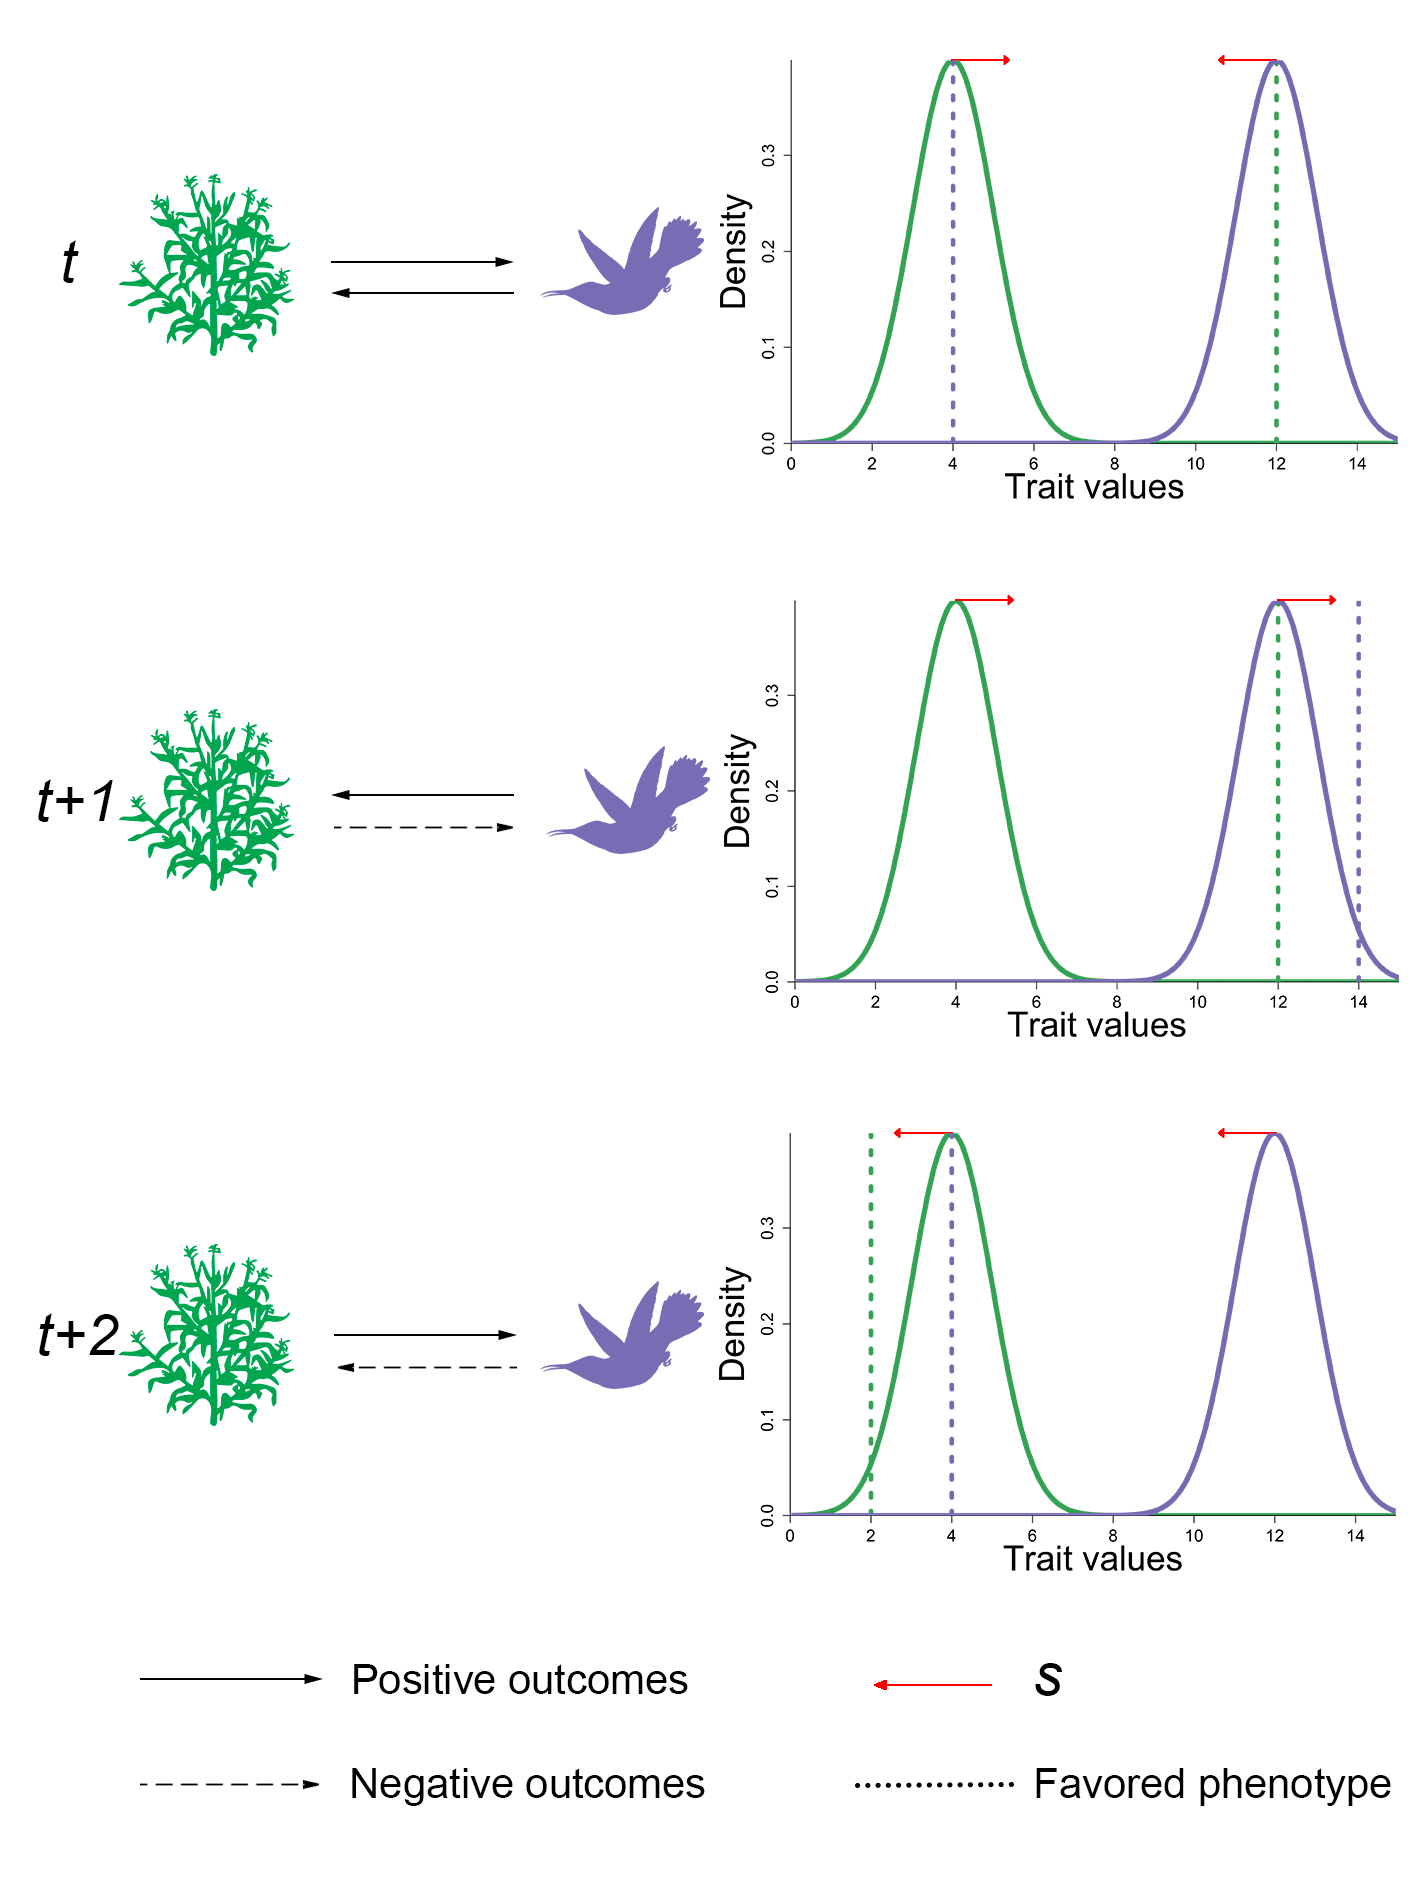
\includegraphics[width=\textwidth]{Fig1_ConDep.png}
\caption{Conceptual figure showing the interaction outcomes changing from a mutualism (t) to an antagonism with different outcome arrangements (t+1 and t+2). There are different favoured phenotypes and selection differentials (s) depending on how the interaction outcomes are arranged. The mutualism promotes trait matching and the antagonism promotes arm's race between the explorer and exploited species.}
\label{fig1}

\end{figure}

\nolinenumbers
\section{References}

\end{document}